\chapter{Metod}
Metodkapitlet beskriver hur arbetsgången i projektet har gått till.

\section{Projektorganisation}
Projektets organisation bestod av sju personer som studerar på Linköpings universitet. Projektet hade även en handledare som fanns tillgänglig om problem skulle uppstå. I detta avsnitt beskrivs hur organisationen var uppbyggd med de olika roller som ingick, hur möten gick till, dokumentation av projektet och ett avsnitt om kompetensutveckling.

\subsection{Roller}
I projektgruppen var varje person tilldelad en specifik roll. Dessa roller innebar att man hade ett antal specifika uppgifter och ansvar att upprätthålla. Nedan beskrivs dessa roller och vad de innebar.

\textbf{Teamledare}\\
Teamledaren har ansvaret för att leda arbetet i gruppen och att gruppen når de mål som har satts upp. För att hjälpa gruppen med detta ska teamledaren arbeta för att coacha gruppen, se till att de processer som är uppsatta efterföljs och se till att gruppen har en trevlig arbetsmiljö.

Teamledaren är även en representant för teamet utåt och är kontaktperson för gruppen mot examinator, handledare eller annan person som kan tänkas vilja ha kontakt med gruppen. Teamledaren har även ansvaret för att en projektplan ska skrivas i förstudien av projektet och har även sista ordet om det skulle uppstå en sådan situation i gruppen.

\textbf{Analysansvarig}\\
Analysansvarig är den person som håller den huvudsakliga kontakten med kunden. Personen tar reda på
vad kunden är ute efter och arbetar därefter med att analysera och sammanställa dessa till en
kravspecifikation för projektet. Om det skulle vara så att krav och behov från kunden är otydliga för 
gruppen är det analysansvariges uppgift att tolka dessa krav åt resten av gruppen så att de är 
förståeliga och så att kunden inte missuppfattas.

För att både projektgruppen och kunden ska bli nöjda är analysansvarig ansvarig för förhandling mellan de båda parterna. Det ska vara en acceptabel kompromiss mellan vad kund vill att projektet ska åstadkomma och vad gruppen tror att man kan åstadkomma. Analysansvarig har mycket kontakt med arkitekten vid utformandet av arkitekturen för produkten, detta så att de krav som är uppsatta blir uppfyllda. Under implementationsfasen ska det finnas en god kontakt med ansvarig testledare. Det är viktigt eftersom när test utförs ska det säkerställas att funktionaliteten och designen stämmer överens med kraven i kravspecifikationen.

\textbf{Arkitekt}\\
Arkitekten har ansvaret för att produkten får en stabil arkitektur. Ansvaret för att göra övergripande teknikval ligger på arkitekten och i tekniska frågor så är det arkitekten som har det sista ordet, bortsett från teamledaren. För att göra dessa teknikval så förväntas det av arkitekten att komponenter och gränssnitt identifieras och att de görs tydliga för gruppen. Denna bakgrundskunskap som arkitekten införskaffar gör att denne är en styrande röst och har möjligheten att kunna kommunicera bärande idéer.

Arkitekten håller en god kontakt med analysansvarig. Detta för att kunna skapa en arkitektur som bygger på och upprätthåller de krav som finns från kunden, men det gäller också att arkitekten genom analysansvarig kommunicerar med kund i de fall det finns krav som inte är möjliga rent kunskaps- eller teknikmässigt.

\textbf{Utvecklingsledare}\\
Utvecklingsledaren har ansvar för att skapa en mer detaljerad design av produkten. Under utvecklingsfasen i projektet så leder och, vid behov, fördelar utvecklingsledaren arbetet så att allting ska gå så smidigt som möjligt. Denna roll har även ansvaret för att fatta beslut om vilken utvecklingsmiljö som ska användas under projektet.

I projektet som hör till denna rapport så är alla i gruppen delaktiga vid utveckling vilket innebär att utvecklingsledaren kommer leda samtliga personer, oavsett vilken roll de innehar.

\textbf{Testledare}\\
Testledaren är den person som ansvarar för att produkten testas enligt en standard som kan säkerställa systemets funktionalitet och uppfyllnad mot de mål som finns uppsatta. För att säkerställa detta och den kvalitet som produkten ska upprätthålla så testas kvalitetskrav tillsammans med kvalitetssamordnaren.

Som testledare är det bra med viss distans till det som testas då beslutet om vilka delar av systemet som anses testade och färdiga ligger hos denna person. Testledaren ansvarar även för att skriva en testplan och en testrapport.

\textbf{Kvalitetssamordnare \& Dokumentansvarig}\\
Den sammanslagna rollen kvalitetssamordnare \& dokumentansvarig går ut på att kunna säkerställa att kvalitet och dokumentation upprätthålls och skrivs under projektets gång. Kvalitetssamordnare tittar på den budget som projektet har och hur mycket av detta man kan lägga på just kvalitet.

Som dokumentansvarig så ser man till att det finns dokumentmallar för de dokument som ska skrivas. Rollen innefattar även ansvar att se till att det tas fram en logotyp för projektet och att gruppen kan leverera till de deadlines som existerar.

Denna sammanslagna roll arbetar mycket med konfigurationsansvarig så att båda är överens om versionshantering och tillvägagångssätt vid produktsläpp.

\textbf{Konfigurationsansvarig}
\\Konfigurationsansvarig har ansvaret för att produkten som skapas versions- och konfigurationshanteras på ett korrekt sätt. Rollen går ut på att bestämma vilka arbetsprodukter som ska versionshanteras och vara med i en specifik utgåva. Då konfigurationsansvarig ser till att version- och konfigurationshantering sköts på ett korrekt sätt så ansvarar denne också för att välja de verktyg som ska användas för versionshanteringen.

Denna roll arbetar mycket med utvecklingsledare och dokumentansvarig då dessa två är ansvariga för utveckling av produkter och dokument som ska ingå i olika utgåvor.

\subsection{Möten}
Gruppen hade möte nästan en gång om dagen för att uppdatera varandra om vad man har gjort, vad man ska göra och om man har några problem. Varannan vecka hade gruppen ett längre möte där man redovisade vad som hade presterats, vad som gått bra/kunde ha gjorts bättre och vad man ska göra under kommande två veckor. Dessa möten följde Scrum-metodik, se avsnitt \ref{scrum}.

Utöver Scrum hade gruppen möte med handledaren en gång i veckan för att uppdatera varandra och handledaren om statusen för projektet. Till dessa möten skickades en dagordning ut av teamledaren i god tid innan mötet. Dagordningen bestod av ett antal punkter som skulle behandlas under handledarmötena. 

Utöver dessa punkter hade medlemmar i projektgruppen samt handledare möjlighet att tillföra punkter på dagordningen, deadline för detta var 12.00 dagen innan respektive möte.
Denna dagordning hade ett antal punkter som alltid togs upp och medlemmar i gruppen samt handledaren kunde skicka in extra punkter att ta upp senast klockan 12.00 dagen innan mötet.

Slutligen höll projektgruppen möten med kund med jämna mellanrum där några personer från projektgruppen träffade några av de involverade personerna på företaget. Dessa möten gick ut på att uppdatera kunden om statusen för projektet, utbyta idéer och se till att projektgruppen och kund var på samma spår.

\subsection{Dokumentation}
För hantering av interna dokument har gruppen främst använt sig av google drive. Detta innefattar bland annat protokoll från handledarmöten, gruppkontrakt, veckorapporter och tidsrapportering.

Externa dokument som har lämnats in i diverse iterationer har gruppen producerat i LaTeX och versionshanterats med hjälp av Git.

\subsection{Kompetensutveckling}
Vid utveckling av kompetens och för att kunna bevara och dela erfarenheter med varandra har gruppen arbetat på några olika sätt.

Om gruppen behövde grundläggande kunskap i något verktyg eller metod gick man tillväga så att en person samlade in kunskap om det aktuella området och sedan höll personen en genomgång för gruppen innan verktyget eller metoden började användas i projektet. Exempelvis så har det varit genomgångar i Git, Scrum och Angular. 

Vidare så ägde dagliga scrum-möten rum där gruppmedlemmarna delade med sig vad de gjort och vilka erfarenheter de fått ut av detta men även samtal och diskussioner fördes mellan gruppmedlarna kontinuerligt. Utöver det så var det upp till var och en att införskaffa den kunskap som behövdes 
för att kunna genomföra projektet.  

\section{Utvecklingsmetod}
I början av projektet hade inte projektgruppen så mycket struktur i arbetet och större delen av gruppen arbetade med konfigurering av diverse verktyg som användes i projektet t.ex. Git, LaTeX och Google Drive.

Efter ett möte med kunden i början av februari kom frågan upp gällande vilket arbetssätt vi skulle använda oss av och kunden föreslog Scrum. Teamledaren i gruppen gjorde efterforskningar om hur Scrum fungerar och gav en presentation för gruppen där slutsatsen var att Scrum fortsättningsvis skulle användas som utvecklingsmetod i projektet.

\section{Förstudie}
\label{sec:forstudie}
Under förstudien, som var uppdelad i två iterationer, arbetade gruppen väldigt mycket med dokumentation som skulle ligga till grund för design och implementation av systemet. Ett flertal dokument utformades. Dessa är listade i tabell 1 nedan.

\begin{table}
\caption{Dokumentation i förstudien}
\begin{tabular}{|c|c|}
\hline
\textbf{Dokument} & \textbf{Beskrivning} \\
\hline
Projektplan & Projekt- och arbetsgång \\
\hline
Kravspecifikation & De krav som finns på produkten \\
\hline
Kvalitetsplan & Försäkring av hög kvalitet i projektet \\
\hline
Statusrapport 1 & Statusrapport över arbetet i iteration 1 \\
\hline
Systemanatomi & Skiss på hur systemet ska se ut \\
\hline
Rapporthalva av kandidatarbetet & Projektet fram till slutet av iteration 2 \\
\hline
Arkitekturdokument & Beskrivning av systemet \\
\hline
Testplan & Hur testning av systemet ska gå till \\
\hline
Testrapport & Testning under iteration 2 \\
\hline
Utvärdering av iteration 2 & Hur arbetet gick under iteration 2 \\
\hline
\end{tabular}
\end{table}

Under iteration två lämnades projektplan, kravspecifikation och kvalitetsplan in en andra gång så att handledaren fick se hur de hade utvecklats.

Utöver denna dokumentation arbetade gruppen mycket med kompetensutveckling för att förstå det system och de verktyg som skulle användas under design- och implementationsfasen. Gruppmedlemmar höll en genomgång av Git och en genomgång av Scrum så gruppen skulle få grundläggande kunskaper och kunna applicera dessa verktyg.

Under förstudien hade gruppen även flera möten med kund för att få information om vad kunden ville ha för typ av produkt så att en kravspecifikation kunde utformas.

\section{Design}
Då kravspecifikationen var färdigställd var det dags för projektet att gå in i designfasen. Under fasen så låg fokus på två saker, grafisk design och mjukvarudesign.

\subsection{Grafisk design}
För att bestämma den grafiska designen av produkten skapade samtliga medlemmar i projektgruppen en egen pappersprototyp på hur man tänkt sig att produkten skulle kunna se ut. Gruppen diskuterade de olika förslagen och slog samman tre alternativ som redovisades för kund.

Kunden gav återkoppling på de olika alternativen och utifrån detta skapade gruppen en ny design och prototyp som efter ett ytterligare möte resulterade i den slutgiltiga designen för produkten.

\subsection{Mjukvarudesign}
Samtidigt som en grafisk design togs fram så arbetade projektets arkitekt och utvecklingsledare på att ta fram designen för mjukvaran. En systemanatomi och en systemskiss skapades för att få en överblick på hur systemet skulle se ut. 


\begin{figure}[H]
    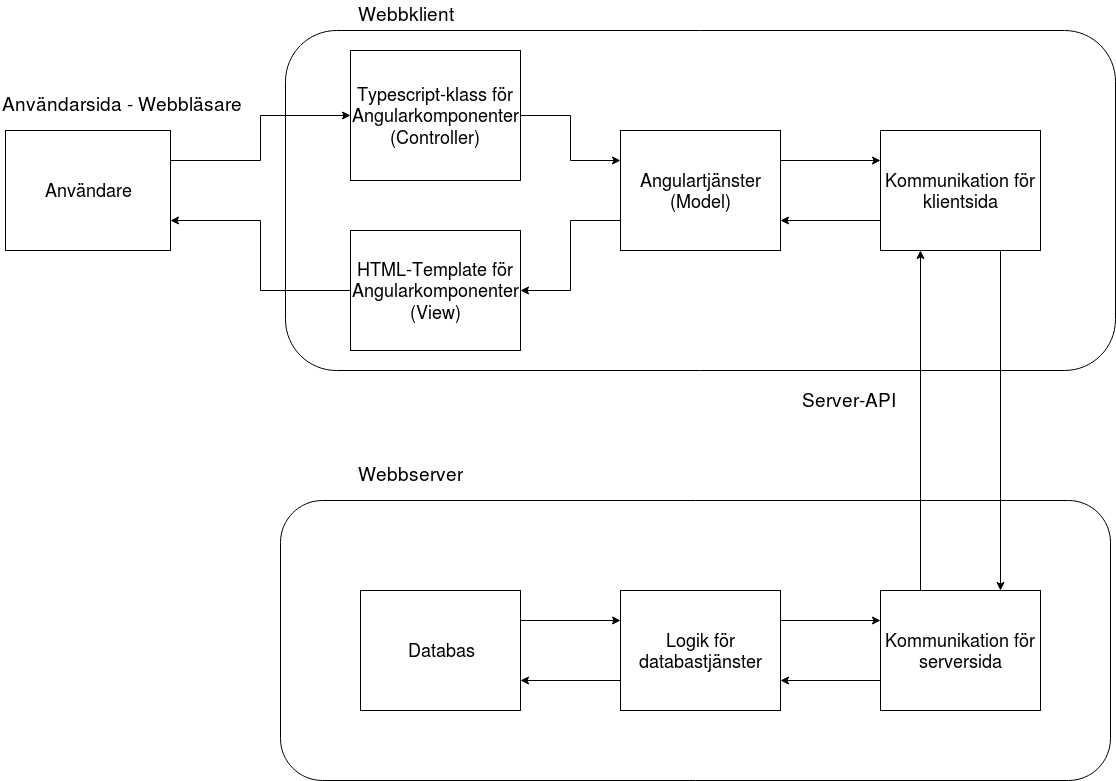
\includegraphics[width=\textwidth,height=.4\textheight]{Figures/Systemskiss.png}\\
    \caption{Systemskiss}
    \label{fig:Systemskiss}
\end{figure}

Det skrevs även ett arkitekturdokument där de olika designbesluten som fattats beskrevs och motiverades. Lösningar som övervägdes men förkastades finns också beskrivna i det dokumentet.

Den mjukvarudesign som togs fram i projektets inledande skede var något översiktlig. Den kompletterades under projektets gång när det blivit klarare vilka mjukvarumässiga problem och utmaningar projektgruppen stod inför. Detta då projektmedlemmarna förvärvade sig ytterligare kunskaper om hur webbutveckling fungerar. 

Besluten om mjukvarudesign fattades ofta utgående från den pappersprototyp som tagits fram i samband med den grafiska designen och demonstrationsmöten med kund.

\section{Utveckling}
När designfasen var över gick gruppen in i projektets utvecklingsfas. Gruppen delades upp i två subgrupper där den ena fokuserade på front-end och den andra på back-end.

\subsection{Front-end}
Arbetet började med att implementera designen för det grafiska gränssnittet med hjälp av Angular komponenter. Efter det så implementerades logiken för de komponenterna. Slutligen sammankopplades det med arbetet gruppen i back-end utfört. Gruppen växlade mellan parprogrammering och enskild programmering beroende på vad som skulle göras.       

\subsection{Back-end}
När utvecklingen av back-end startade skapades först ett EER-diagram över den databas som produkten skulle använda sig av för att lagra data. 
Sedan översattes diagrammet till kod, som skrevs i Javascript med hjälp av Sequelize. 
Gruppen skrev ett API som också implementerades i back-end koden så att man enkelt skulle kunna hämta och modifiera data i databasen.

\section{Utvärdering}
Under projektets gång så utvärderade gruppen arbetet kontinuerligt. Gruppen gjorde även en utvärdering i slutet av projektet.

\subsection{Sprintutvärdering}
Gruppen arbetade med tvåveckors-sprintar, vilket innebar att det gjordes en sprintutvärdering varannan vecka. Under utvärderingen gick gruppen igenom vad som hade gått bra under de två veckor som gått och vad som inte gick lika bra. Gruppen listade vad som hade kunnat förbättras och valde sedan ut 2-3 punkter att arbeta med under nästkommande sprint. Gruppen diskuterade även hur arbetet hade gått med de punkter man arbetat med under föregående sprint.

\subsection{Utvärdering av projektet}
I slutet av arbetet utförde gruppen en utvärdering av projektet i sin helhet. Där reflekterade gruppen över resultatet, hur arbetet hade gått och vad man hade kunnat göra bättre.
